
Das ERP-KMU-Fit-Modell konzentriert sich auf Voraussetzungen, die vor Beginn
der Implementierung in ausreichendem Maß vorhanden sein müssen. Es beschreibt
damit nicht die späteren Wirkungen eines bereits genutzten ERP-Systems, sondern
die Implementierungsbereitschaft eines KMU. Die einzelnen Fit-Dimensionen
wirken dabei nicht unabhängig voneinander, sondern greifen in der Vorbereitung
eines ERP-Projekts ineinander.

Den Ausgangspunkt bilden Strategie-Fit, Kompetenz-Fit und Ressourcen-Fit.
Diese drei Dimensionen schaffen gemeinsam die Grundlage für die
Projektvorbereitung. Der Strategie-Fit konkretisiert, welchen strategischen
Beitrag das ERP-System leisten soll, welche Ziele verfolgt werden und welche
Anforderungen daraus für Projektumfang und Systemauswahl entstehen. Eine klare
strategische Orientierung schafft damit die Grundlage für ein realistisch
abgegrenztes ERP-Projekt und für die Auswahl einer zum Unternehmen passenden
Lösung \parencite{Leyh2015,Jha2008}.

Der Ressourcen-Fit beschreibt, ob ausreichende finanzielle, personelle und
zeitliche Kapazitäten für die Vorbereitung und Durchführung des Projekts
vorhanden sind. Die Verfügbarkeit von Ressourcen bestimmt damit, ob zentrale Vorarbeiten wie Ist-Analyse,
Projektplanung, Prozessaufnahme und Datenbereinigung mit ausreichender
Sorgfalt durchgeführt werden können \parencite{Leyh2015,Jha2008}.

Der Kompetenz-Fit ergänzt diese Ressourcen um das notwendige Wissen für
Analyse, Auswahl und Planung. Dazu gehören insbesondere Prozessverständnis,
ERP- und IT-Wissen sowie Projektmanagementkompetenz. Nur wenn das KMU über
dieses Wissen verfügt oder es gezielt einbinden kann, lassen sich strategische
Ziele in konkrete Anforderungen an das ERP-System überführen
\parencite{Leyh2015,Jha2008}.

Strategie-Fit, Kompetenz-Fit und Ressourcen-Fit münden somit in die
ERP-Vorbereitung. In dieser Phase werden die bestehenden Abläufe analysiert,
Anforderungen formuliert, das Projekt geplant und die Einführung vorbereitet.
Auf dieser Grundlage werden Prozess-Fit und Daten-Fit bewertet.

Der Prozess-Fit zeigt, ob zentrale Unternehmensabläufe ausreichend klar und
nachvollziehbar sind, um daraus Anforderungen abzuleiten und eine passende
Systemkonfiguration vorzubereiten. Er wird im Rahmen der Ist-Analyse
bewertet. Die Analyse und gegebenenfalls erforderliche Anpassung von Prozessen
setzt wiederum eine klare strategische Orientierung sowie ausreichende
finanzielle, personelle und fachliche Ressourcen voraus \parencite{Leyh2015}.

Der Daten-Fit beschreibt dagegen, ob relevante Unternehmensdaten in
ausreichender Qualität, Konsistenz und Struktur vorliegen, damit sie in das
ERP-System überführt werden können. Auch hierfür ist ein strukturiertes
Vorgehen zur Datenerhebung, Bereinigung und Vereinheitlichung erforderlich \parencite{Leyh2015}.
Nur so kann die vorhandene Datenqualität bewertet und, soweit notwendig, vor
der Implementierung verbessert werden.

\begin{figure}[htbp]
  \centering
  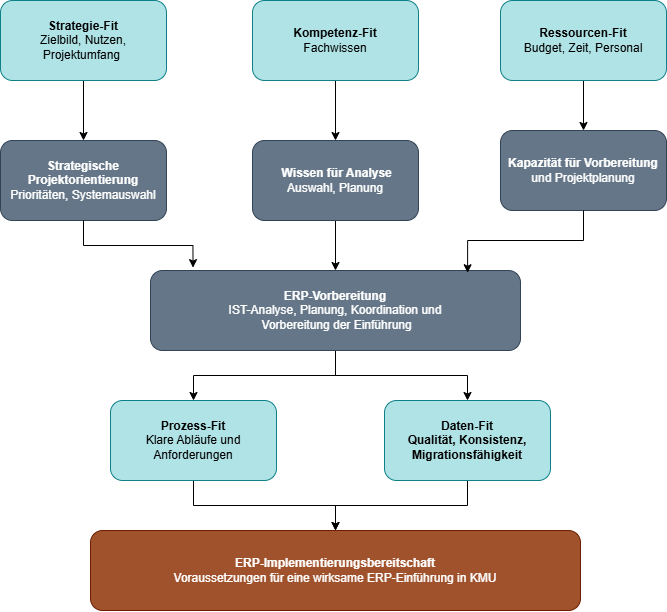
\includegraphics[
    width=\textwidth,
    keepaspectratio
  ]{figures/erp-kmu-fit-modell.png}
  \caption{Wirklogik des ERP-KMU-Fit-Modells, eigene Darstellung auf Basis
  der ausgewerteten Literatur}
  \label{fig:erp-kmu-fit-modell}
\end{figure}

ERP-Implementierungsbereitschaft liegt vor, wenn alle fünf Fit-Dimensionen in
einem ausreichenden Mindestmaß erfüllt sind. Defizite in einer Dimension können
dabei die Vorbereitung in anderen Bereichen beeinträchtigen. Fehlende
Ressourcen können beispielsweise die Prozessanalyse oder Datenbereinigung
erschweren, während fehlendes Wissen eine unpassende Systemauswahl oder eine
unzureichende Projektplanung begünstigen kann.
